\documentclass{article}

\usepackage{fancyhdr}
\usepackage{extramarks}
\usepackage{amsmath}
\usepackage{amsthm}
\usepackage{amsfonts}
\usepackage{tikz}
\usepackage[plain]{algorithm}
\usepackage{algpseudocode}
\usepackage{enumerate}
\usepackage{mathtools}
\usepackage{enumitem}

\usetikzlibrary{automata,positioning}

%
% Basic Document Settings
%

\topmargin=-0.45in
\evensidemargin=0in
\oddsidemargin=0in
\textwidth=6.5in
\textheight=9.0in
\headsep=0.25in

\linespread{1.1}

\pagestyle{fancy}
\lhead{\hmwkAuthorName}
\chead{\hmwkClass\ (\hmwkClassInstructor\ \hmwkClassTime): \hmwkTitle}
\rhead{\firstxmark}
\lfoot{\lastxmark}
\cfoot{\thepage}

\renewcommand\headrulewidth{0.4pt}
\renewcommand\footrulewidth{0.4pt}

\setlength\parindent{0pt}

%
% Create Problem Sections
%

\newcommand{\enterProblemHeader}[1]{
    \nobreak\extramarks{}{Problem \arabic{#1} continued on next page\ldots}\nobreak{}
    \nobreak\extramarks{Problem \arabic{#1} (continued)}{Problem \arabic{#1} continued on next page\ldots}\nobreak{}
}

\newcommand{\exitProblemHeader}[1]{
    \nobreak\extramarks{Problem \arabic{#1} (continued)}{Problem \arabic{#1} continued on next page\ldots}\nobreak{}
    \stepcounter{#1}
    \nobreak\extramarks{Problem \arabic{#1}}{}\nobreak{}
}

\setcounter{secnumdepth}{0}
\newcounter{partCounter}
\newcounter{homeworkProblemCounter}
\setcounter{homeworkProblemCounter}{1}
\nobreak\extramarks{Problem \arabic{homeworkProblemCounter}}{}\nobreak{}

%
% Homework Problem Environment
%
% This environment takes an optional argument. When given, it will adjust the
% problem counter. This is useful for when the problems given for your
% assignment aren't sequential. See the last 3 problems of this template for an
% example.
%
\newenvironment{homeworkProblem}[1][-1]{
    \ifnum#1>0
    \setcounter{homeworkProblemCounter}{#1}
    \fi
    \section{Problem \arabic{homeworkProblemCounter}}
    \setcounter{partCounter}{1}
    \enterProblemHeader{homeworkProblemCounter}
    }{
    \exitProblemHeader{homeworkProblemCounter}
}

%
% Homework Details
%   - Title
%   - Due date
%   - Class
%   - Section/Time
%   - Instructor
%   - Author
%

\newcommand{\hmwkTitle}{Problem Set\ \#2}
\newcommand{\hmwkDueDate}{February 6, 2017}
\newcommand{\hmwkClass}{MATH 327}
\newcommand{\hmwkClassInstructor}{Professor Mei-Hsiu Chen}
\newcommand{\hmwkAuthorName}{Tim Hung}

%
% Title Page
%

\title{
    \vspace{2in}
    \textmd{\textbf{\hmwkClass:\ \hmwkTitle}}\\
    \normalsize\vspace{0.1in}\small{Due\ on\ \hmwkDueDate\ at 1:10pm}\\
    \vspace{0.1in}\large{\textit{\hmwkClassInstructor\ \hmwkClassTime}}\\
}

\author{\textbf{\hmwkAuthorName}}
\date{}

\renewcommand{\part}[1]{\textbf{\large Part \Alph{partCounter}}\stepcounter{partCounter}\\}

%
% Various Helper Commands
%

% Useful for algorithms
\newcommand{\alg}[1]{\textsc{\bfseries \footnotesize #1}}

% For derivatives
\newcommand{\deriv}[1]{\frac{\mathrm{d}}{\mathrm{d}x} (#1)}

% For partial derivatives
\newcommand{\pderiv}[2]{\frac{\partial}{\partial #1} (#2)}

% Integral dx
\newcommand{\dx}{\mathrm{d}x}

% Alias for the Solution section header
\newcommand{\solution}{\textbf{\large Solution}}

% Probability commands: Expectation, Variance, Covariance, Bias
\newcommand{\E}{\mathrm{E}}
\newcommand{\Var}{\mathrm{Var}}
\newcommand{\Cov}{\mathrm{Cov}}
\newcommand{\Bias}{\mathrm{Bias}}

\begin{document}

\maketitle

\pagebreak

\begin{homeworkProblem}
    A box contains three marbles — one red, one green, and one blue. Consider an
    experiment that consists of taking one marble from the box, then replacing it in the box and drawing a second marble from the box. Describe the sample space.  Repeat for the case in which the second marble is drawn without first replacing the first marble.\\

    \textbf{With replacement}
    \[A = \{RR, RB, RG, BR, BB, BG, GR, GB, GG\}\]

    \textbf{Without replacement}
    \[B = A \setminus \{RR, BB, GG\}\]

\end{homeworkProblem}

\begin{homeworkProblem}[3]
    Let $S = \{1, 2, 3, 4, 5, 6, 7\}$, $E = \{1, 3, 5, 7\}$, $F = \{7, 4, 6\}$, $G = \{1, 4\}$. Find

    \begin{enumerate}[label=(\alph*)]
        \item $ EF = \{7\}$
        \item $ E\cup FG = \{1,3,4,5,7\}$
        \item $ EG^c = \{3,5,7\}$
        \item $ EF^c \cup G = \{1,3,4,5\}$
        \item $ E^{c}(F\cup G) = \{4,6\}$
        \item $ EG\cup FG = \{1,4\}$
    \end{enumerate}
\end{homeworkProblem}

\begin{homeworkProblem}[7]
    Find simple expressions for the events
    \begin{enumerate}[label=(\alph*)]
        \item $ E\cup E^c = \emptyset ^c$
        \item $ EE^c = \emptyset$
        \item $ (E\cup F)(E\cup F^c) = E$
        \item $ (E\cup F)(E^c \cup F)(E\cup F^c) = E\cap F$
        \item $ (E\cup F)(F\cup G) = F\cup (E\cap G)$
    \end{enumerate}
\end{homeworkProblem}

\pagebreak

\begin{homeworkProblem}[9]
    For the following Venn diagram, describe in terms of E, F, and G the events
    denoted in the diagram by the Roman numerals I through VII.

    \begin{center}
    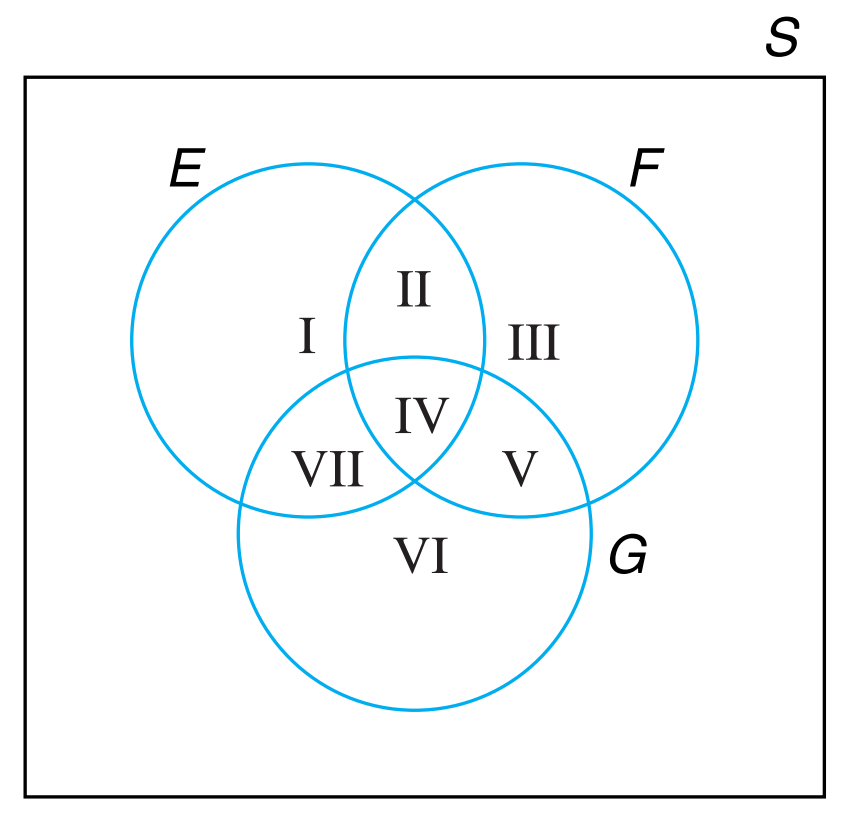
\includegraphics[width=8cm]{3-9.png}
    \end{center}

    \begin{enumerate}[label=(\Roman*)]
        \item $S\setminus (F\cup G)$
        \item $(E\cap F)\setminus G$
        \item $S\setminus (E\cup G)$
        \item $E\cap F\cap G$
        \item $(F\cap G)\setminus E$
        \item $S\setminus (E\cup F)$
        \item $(E\cap G)\setminus F$
    \end{enumerate}
\end{homeworkProblem}

\begin{homeworkProblem}[12]
    If $P(E) = .9$ and $P(F) = .9$, show that $P(EF ) \geq .8$. In general, prove Bonferroni's inequality, namely that
    \[ P(EF) \geq P(E) + P(F) - 1 \]
    \textbf{Solution}
    \[ 1 \geq P(E\cup F) = P(E) + P(F) - P(E\cap F)\]
\end{homeworkProblem}

\begin{homeworkProblem}[15]
    Calculate $\binom{9}{3},\binom{9}{6},\binom{7}{2},\binom{7}{5}, \binom{10}{7}$.
    \[
        \binom{9}{3} = 84, 
        \binom{9}{6} = 84,
        \binom{7}{2} = 21,
        \binom{7}{5} = 21,
        \binom{10}{7} = 120
    \]
\end{homeworkProblem}

\begin{homeworkProblem}[21]
    There is a 60 percent chance that the event A will occur. If A does not occur, then
    there is a 10 percent chance that B will occur.
    \begin{enumerate}[label=(\alph*)]
        \item
            What is the probability that at least one of the events A or B occurs?
            \[
                P(A\cup B) = P(A\cup B \mid A)P(A) + P(A\cup B\mid A^c )P(A^c) = P(A) + P(B\mid A^c)P(A^c) = .6 + .1 \times .4 = .64
            \]
        \item
            If A is the event that the democratic candidate wins the presidential election in 2012 and B is the event that there is a 6.2 or higher earthquake in Los Angeles sometime in 2013, what would you take as the probability that both A and B occur? What assumption are you making?
            \[P(A\cap B) = .6 \times .1 = .06\]
    \end{enumerate}
\end{homeworkProblem}

\begin{homeworkProblem}[25]
    Fifty-two percent of the students at a certain college are females. Five percent of the students in this college are majoring in computer science. Two percent of the students are women majoring in computer science. If a student is selected at random, find the conditional probability that
    \begin{enumerate}[label=(\alph*)]
        \item
            this student is female, given that the student is majoring in computer science;

            Let $P(F)$ be the probability that a student is female.

            Let $P(C)$ be the probability that a student studies CS.
            \[P(F\mid C) = \frac{P(F\cap C)}{P(C)} = \frac{.02}{.05} = .4\]
        \item
            this student is majoring in computer science, given that the student is female.
            \[P(C\mid F) = \frac{P(C\cap F)}{P(F)} = \frac{.02}{.52} = .038...\]
    \end{enumerate}
\end{homeworkProblem}

\pagebreak

\begin{homeworkProblem}[34]
    Prostate cancer is the most common type of cancer found in males. As an indicator of whether a male has prostate cancer, doctors often perform a test that measures the level of the PSA protein (prostate specific antigen) that is produced only by the prostate gland. Although higher PSA levels are indicative of cancer, the test is notoriously unreliable. Indeed, the probability that a noncancerous man will have an elevated PSA level is approximately .135, with this probability increasing to approximately .268 if the man does have cancer. If, based on other factors, a physician is 70 percent certain that a male has prostate cancer, what is the conditional probability that he has the cancer given that

    \begin{enumerate}[label=(\alph*)]
        \item
            the test indicates an elevated PSA level

            Let $P(C) = .7$ be the probability that a male has prostate cancer.

            Let $P(E)$ be the probability that a male has an elevated PSA level.

            \[
                P(C|E) = \frac{P(C\cap E)}{P(E)} 
                = \frac{P(E|C)P(C)}{P(E|C)P(C)+P(E|C^c)P(C^c)}
                = \frac{.268 \times .7}{.268 \times .7 + (.135)(1-.7)}
                = .822..
            \]

        \item
            the test does not indicate an elevated PSA level
            \[
                P(C|E^c) = \frac{P(C\cap E^c)}{P(E^c)} 
                = \frac{P(E^c|C)P(C)}{P(E^c|C)P(C)+P(E^c|C^c)P(C^c)}
                = \frac{(1-.268)(.7)}{(1-.268)(.7) + (1-.135)(1-.7)}
                = .664...
            \]
    \end{enumerate}
    Repeat the preceding, this time assuming that the physician initially believes there is a 30 percent chance the man has prostate cancer.
    \begin{enumerate}[label=(\alph*)]
        \item
            the test indicates an elevated PSA level

            Let $P(C) = .3$ be the probability that a male has prostate cancer.

            Let $P(E)$ be the probability that a male has an elevated PSA level.
            \[
                P(C|E) = \frac{P(C\cap E)}{P(E)} 
                = \frac{P(E|C)P(C)}{P(E|C)P(C)+P(E|C^c)P(C^c)}
                = \frac{.268 \times .3}{.268 \times .3 + (.135)(1-.3)}
                = .460..
            \]

        \item
            the test does not indicate an elevated PSA level
            \[
                P(C|E^c) = \frac{P(C\cap E^c)}{P(E^c)} 
                = \frac{P(E^c|C)P(C)}{P(E^c|C)P(C)+P(E^c|C^c)P(C^c)}
                = \frac{(1-.268)(.3)}{(1-.268)(.3) + (1-.135)(1-.3)}
                = .266...
            \]
    \end{enumerate}
\end{homeworkProblem}

\pagebreak

\begin{homeworkProblem}[41]
    A parallel system functions whenever at least one of its components works.  Consider a parallel system of n components, and suppose that each component independently works with probability $\frac{1}{2}$ . Find the conditional probability that component 1 works, given that the system is functioning.

    Let P(C) be the probability that component 1 works.

    Let P(F) be the probability that the system is functioning.
    \[
        P(C|F)=\frac{P(C\cap F)}{P(F)} = \frac{P(F|C)(.5)}{1-.5^n} = \frac{.5}{1-.5^n}
    \]
\end{homeworkProblem}

\begin{homeworkProblem}[42]
    A certain organism possesses a pair of each of 5 different genes (which we will designate by the first 5 letters of the English alphabet). Each gene appears in 2 forms (which we designate by lowercase and capital letters). The capital letter will be assumed to be the dominant gene in the sense that if an organism possesses the gene pair xX, then it will outwardly have the appearance of the X gene. For instance, if X stands for brown eyes and x for blue eyes, then an individual having either gene pair XX or xX will have brown eyes, whereas one having gene pair xx will be blue-eyed. The characteristic appearance of an organism is called its phenotype, whereas its genetic constitution is called its genotype. (Thus 2 organisms with respective genotypes aA, bB, cc, dD, ee and AA, BB, cc, DD, ee would have different genotypes but the same phenotype.) In a mating between 2 organisms each one contributes, at random, one of its gene pairs of each type. The 5 contributions of an organism (one of each of the 5 types) are assumed to be independent and are also independent of the contributions of its mate. In a mating between organisms having genotypes aA, bB, cC, dD, eE, and aa, bB, cc, Dd, ee, what is the probability that the progeny will (1) phenotypically, (2) genotypically resemble
    \begin{enumerate}
        \item Phenotypically
            \begin{enumerate}[label=(\alph*)]
            \item the first parent
                \[.5\times .75\times .5\times .75\times .5 = .07...\]
            \item the second parent
                \[.5\times .75\times .5\times .75\times .5 = .07...\]
            \item either parent
                \[.07 + .07 = .14...\]
            \item neither parent
                \[1-.14 = .86...\]
        \end{enumerate}
        \item Genotypically
            \begin{enumerate}[label=(\alph*)]
            \item the first parent
                \[.5\times .5\times .5\times .5\times .5\times = .031...\]
            \item the second parent
                \[.5\times .5\times .5\times .5\times .5\times = .031...\]
            \item either parent
                \[.031... + .031... = .625\]
            \item neither parent
                \[1-.625 = .938...\]
        \end{enumerate}

    \end{enumerate}
\end{homeworkProblem}

\begin{homeworkProblem}[47]
    Let A, B, C be events such that P(A) = .2, P(B) = .3, P(C) = .4.
    Find the probability that at least one of the events A and B occurs if
    \begin{enumerate}[label=(\alph*)]
        \item A and B are mutually exclusive;
            \[P(A) + P(B) = .2 + .3 = .5\]
        \item A and B are independent.
            \[P(A) + P(B) - P(A)P(B) = .2 + .3 - .2 \times .3 = .44\]
    \end{enumerate}

    Find the probability that all of the events A, B, C occur if

    \begin{enumerate}[label=(\alph*), start=3]
        \item A, B, C are independent;
            \[P(A)P(B)P(C) = .2\times .3\times .4 = .024\]
        \item A, B, C are mutually exclusive.
            \[0\]
    \end{enumerate}
\end{homeworkProblem}

\begin{homeworkProblem}[48]
    Two percent of woman of age 45 who participate in routine screening have breast cancer. Ninety percent of those with breast cancer have positive mammographies.  Ten percent of the women who do not have breast cancer will also have positive mammographies. Given a woman has a positive mammography, what is the probability she has breast cancer?\\

    Let P(C) be the probability that a woman has breast cancer.

    Let P(M) be the probability that a woman has a positive mammography.

    \[
        P(C|M)
        = \frac{P(C\cap M)}{P(M)}
        = \frac{P(M|C)P(C)}{P(M|C)P(C)+P(M|C^c)P(C^c)}
        = \frac{.9\times .2}{.9\times .02 + (.1)(1-.02)}
        = .155
    \]
\end{homeworkProblem}

\pagebreak

\section{In Class \#1}
\enterProblemHeader{1} {

    Prove the following statement. If E and F are independent, $E^c$ and $F^c$ are also independent.\\

    Let E and F be independent. If $E^c$ and $F^c$ are also independent, then it suffices to prove that 
    \[P(E^c \cap F^c) = P(E^c)\cdot P(F^c)\]

    Proof

    \begin{center}
    \begin{align}
        P(E^c \cap F^c) &= P((E\cup F)^c)\\
                        &= 1 - P(E\cup F)\\
                        &= 1 - (P(E) + P(F) - P(E\cap F))\\
                        &= 1 - (P(E) + P(F) - P(E)\cdot P(F))\\
                        &= (1 - P(E)) - P(F)(1 - P(E)))\\
                        &= (1-P(E))\cdot (1-P(F))\\
                        &= P(E^c)\cdot P(F^c)
    \end{align}
    \end{center}

\exitProblemHeader{1}}

\section{In Class \#2}
\enterProblemHeader{Problem 2} {
    $E\subset F$. Express $P(E^c \cap F)$ in terms of $P(E)$, $P(F)$, $P(E^c)$, or $P(F^c)$.

    \[
        P(E^c \cap F) = P(F) - P(E)
    \]
\exitProblemHeader{2}}

\end{document}
